\documentclass{egpubl}
\usepackage{eurovis2014}

% --- for  Annual CONFERENCE
\ConferenceSubmission   % uncomment for Conference submission
% \ConferencePaper        % uncomment for (final) Conference Paper
% \STAR                   % uncomment for STAR contribution
% \Tutorial               % uncomment for Tutorial contribution
% \ShortPresentation      % uncomment for (final) Short Conference Presentation
% \Areas                  % uncomment for Areas contribution
% \MedicalPrize           % uncomment for Medical Prize contribution
% \Education              % uncomment for Education contribution
%
% --- for  CGF Journal
% \JournalSubmission    % uncomment for submission to Computer Graphics Forum
% \JournalPaper         % uncomment for final version of Journal Paper
%
% --- for  CGF Journal: special issue
%\SpecialIssueSubmission    % uncomment for submission to Computer Graphics Forum, special issue
% \SpecialIssuePaper         % uncomment for final version of Journal Paper, special issue
%
% --- for  EG Workshop Proceedings
% \WsSubmission    % uncomment for submission to EG Workshop
% \WsPaper         % uncomment for final version of EG Workshop contribution
%
 \electronicVersion % can be used both for the printed and electronic version

% !! *please* don't change anything above
% !! unless you REALLY know what you are doing
% ------------------------------------------------------------------------

% for including postscript figures
% mind: package option 'draft' will replace PS figure by a filname within a frame
\ifpdf \usepackage[pdftex]{graphicx} \pdfcompresslevel=9
\else \usepackage[dvips]{graphicx} \fi

\PrintedOrElectronic

% prepare for electronic version of your document
\usepackage{t1enc,dfadobe}

\usepackage{egweblnk}
\usepackage{cite}
\usepackage[usenames,dvipsnames,svgnames]{xcolor}
\usepackage{subfigure}
\usepackage{flushend}
\usepackage[compact]{titlesec}
\usepackage[normalem]{ulem}
\usepackage{titlesec}

\def\etal{\textit{et al.}}
\renewcommand\floatpagefraction{1.0}
\renewcommand\topfraction{1.0}
\renewcommand\bottomfraction{.9}
\renewcommand\textfraction{.1}
\setcounter{totalnumber}{20}
\setcounter{topnumber}{10}
\setcounter{bottomnumber}{10}
\definecolor{MyGreen}{rgb}{0,0.7,0}
\definecolor{MyWhite}{rgb}{1,1,1}
\definecolor{MyGray}{rgb}{0.5,0.5,0.5}
\definecolor{LightGray}{rgb}{0.7,0.7,0.7}
\definecolor{DarkGray}{rgb}{0.3,0.3,0.3}
\definecolor{DarkYellow}{rgb}{0.7,0.7,0.0}
\definecolor{MyNavyBlue}{rgb}{0.2,0.3,0.7}
\definecolor{darkgreen}{rgb}{0,0.55,0}
\newcommand{\black}[1]{{\color{Black} #1}}
\newcommand{\white}[1]{{\color{MyWhite} #1}}
\newcommand{\gray}[1]{{\color{MyGray} #1}}
\newcommand{\red}[1]{{\color{red} #1}}
\newcommand{\green}[1]{{\color{MyGreen} #1}}
\newcommand{\blue}[1]{{\color{MyNavyBlue} #1}}
\newcommand{\yellow}[1]{{\color{DarkYellow} #1}}
\newcommand{\maybe}[1]{\yellow{#1}}
\newcommand{\rout}[1]{\red{\sout{#1}}}
\newcommand{\repl}[2]{\rout{#1} \green{#2}}
\newcommand{\fix}[1]{\red{\emph{(#1)}}}
\newcommand{\Fix}[1]{\begin{itemize} \renewcommand\labelitemi{\red{--}} \item \red{#1} 
\end{itemize}}

\newcommand{\todo}[1] {\textbf{[~}\textcolor {red}{#1}\marginpar{\textcolor {red}{\centerline{{\Huge \textbf{!}}}}}\textbf{~]}}
\newcommand{\question}[1] {\textbf{[~}\textcolor {darkgreen}{#1}\marginpar{\textcolor {darkgreen}{\centerline{{\Huge \textbf{!}}}}}\textbf{~]}}
\newcommand{\diff}[1]{[\textcolor{blue}{#1}\marginpar{\textcolor{blue}{\centerline{{\Huge \textbf{!}}}}}]}


\def\IC{IC}
\def\SAR{SAR}
\def\USAR{USAR}

\setlength\fboxsep{0pt}
\setlength{\textfloatsep}{8.5pt}
%\setlength{\dbltextfloatsep}{15pt}
%\setlength{\parskip}{4pt}
%\setlength{\parindent}{1em}

% end of prologue

%% Paper title.
\title[Decision-Support for Urban Search \& Rescue Planning]{Decision-Support for Urban Search \& Rescue Mission Planning through Visualization-Based Analysis}

\author[\#255]{Submission ID \#255}
%\author[A. Bock et al.] {
%    Alexander Bock$^1$, Jonas Lundberg$^2$, Alexander Kleiner$^3$, and Timo Ropinski$^1$ \\
%    $^1$ Scientific Visualization Group, Link\"oping University, Sweden\\
%    $^2$ Graphic Design Group, Link\"oping University, Swerden\\
%    $^3$ Collaborative Robotics Group, Link\"oping University, Sweden
%    }

\teaser{
	\centering
	\subfigure[Office fly-through. Enabling the operator to form a insight of the damaged structure.]{\fbox{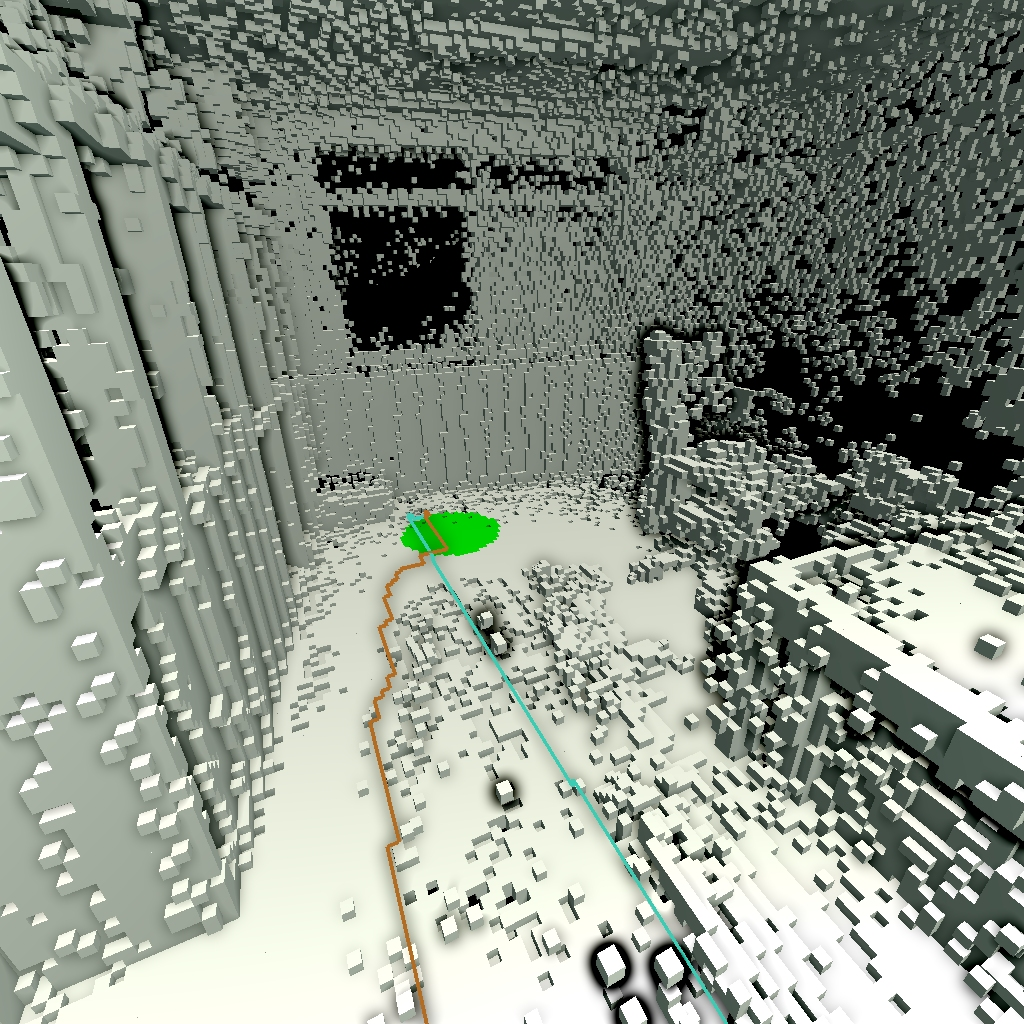
\includegraphics[height=0.25\linewidth]{figures/image1.jpg}}\label{fig:teaser:1}}
	\hfill
	\subfigure[Two of the viable paths in a corridor with two hazardous environments.]{\fbox{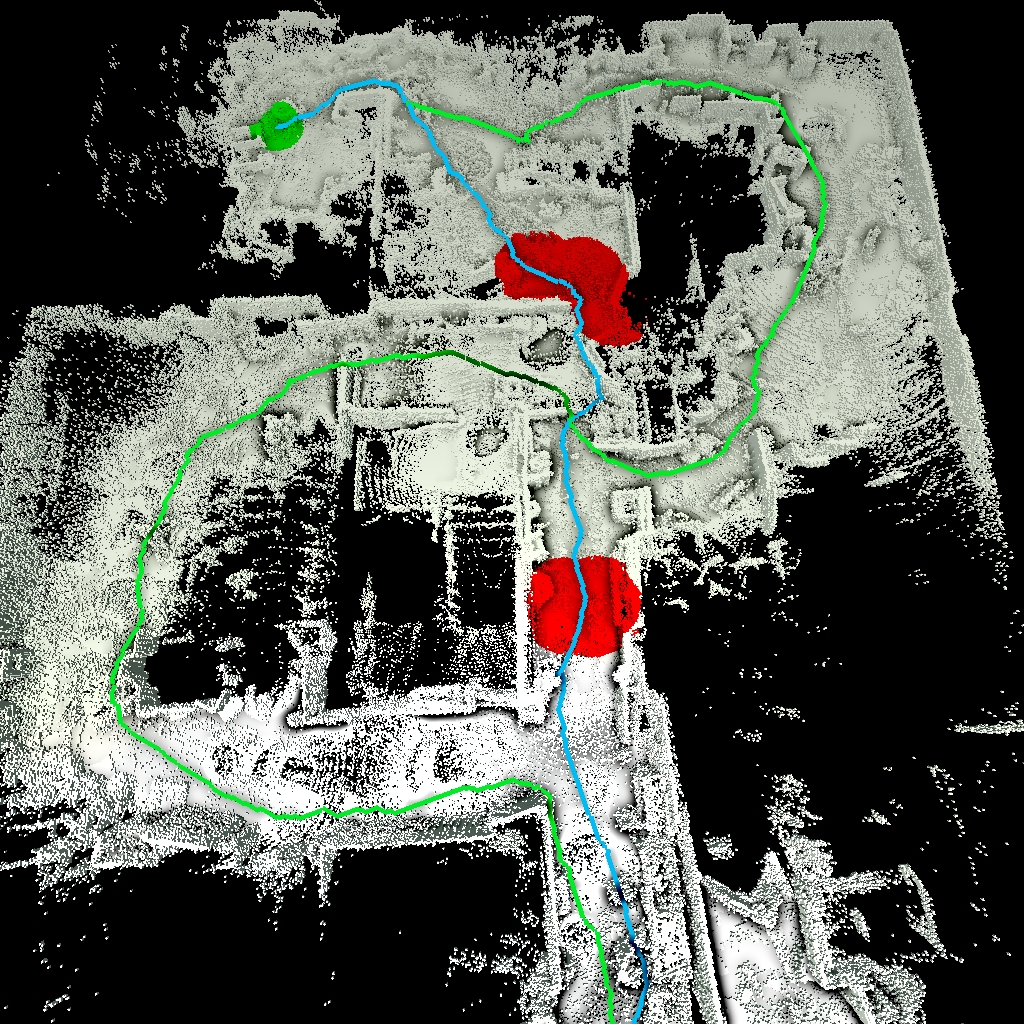
\includegraphics[height=0.25\linewidth]{figures/image2.jpg}}\label{fig:teaser:2}}
	\hfill
	\subfigure[Overhead view of the area in (b) providing context.]{\fbox{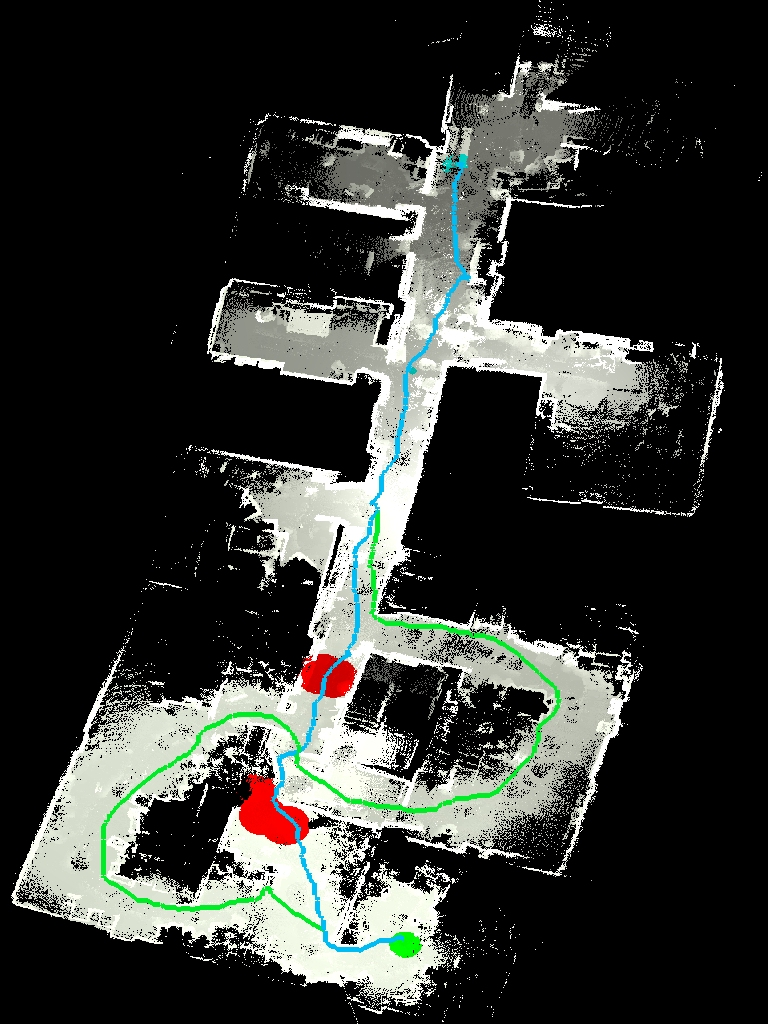
\includegraphics[height=0.25\linewidth]{figures/image2-overview.jpg}}\label{fig:teaser:3}}
	\hfill
	\subfigure[In-depth analysis of an ensemble of paths using parallel coordinates plots and profile plots.]{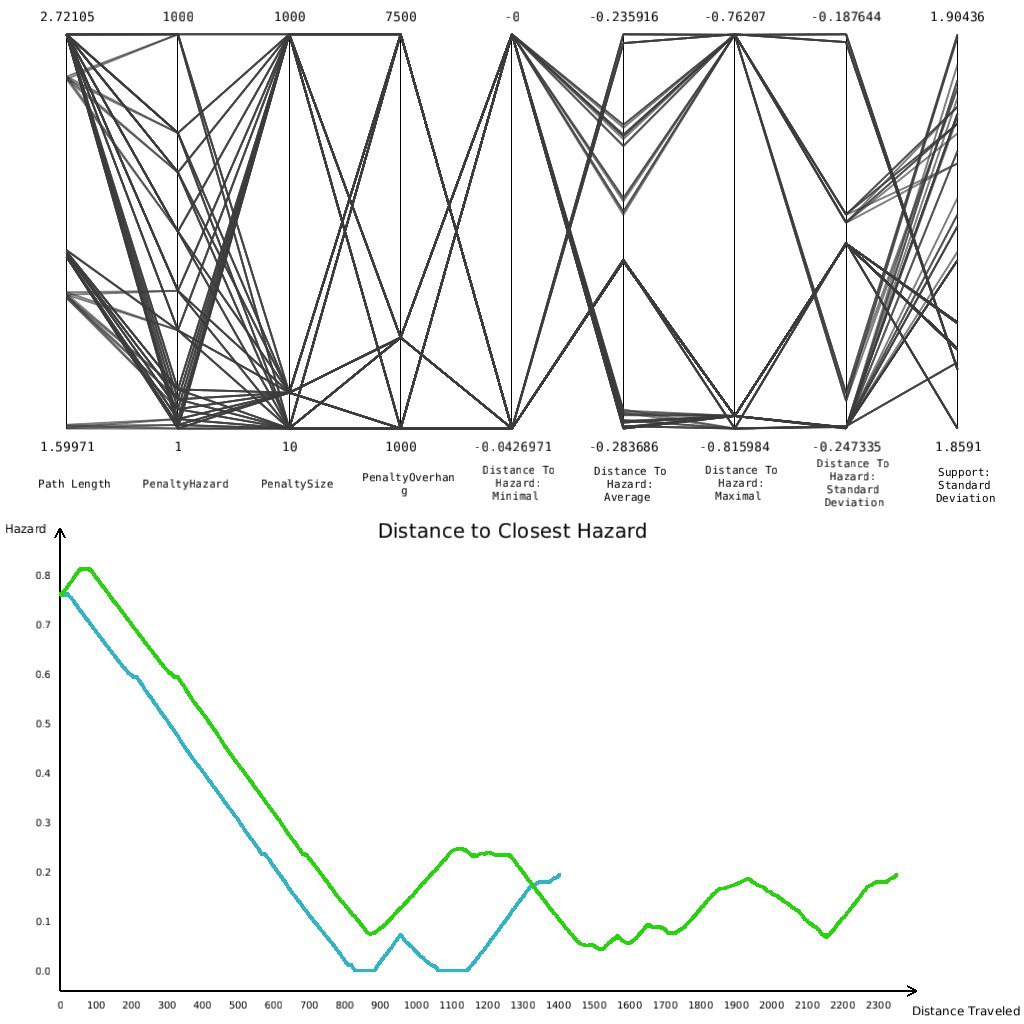
\includegraphics[height=0.25\linewidth]{figures/image4-combined.jpg}\label{fig:teaser:4}}
    \caption{Our visualization system as applied to path planning in the Fukushima Daiichi nuclear reactor site. Different views (a--c) present the operator with a comprehensive understanding of the building, allowing him to select between paths to reach a point-of-interest. The assessment of the trade-off between the paths is supported by a set of visual analysis tools (d).}
    \label{fig:teaser}
}

\begin{document}
\maketitle

\begin{abstract}
We propose a visualization system for incident commanders in urban search~\&~rescue scenarios that supports access path planning for post-disaster structures. Utilizing point cloud data acquired from unmanned robots, we combine visualization with visual analytics methods to allow for assessment of automatically generated access paths. Uncertainty in the data and a priori unknown information make fully automated systems impractical for this problem, thus requiring human interaction. To this end, we present a set of viable access paths, computed based on varying risk factors, to the incident commander in a three-dimensional environment combined with visual analysis tools to inspect paths in detail and make informed decisions. Based on this decision, a responder is guided along the path by the incident commander, who can interactively annotate and reevaluate the acquired point cloud. We describe design considerations for our system, its technical realization, and discuss the results of an expert evaluation.
\end{abstract}
\vspace*{-0.75cm}

\section{Introduction}
Natural and man-made disasters causing structural damage to inhabited buildings are an ever-present danger. As time-to-rescue is one of the most important factors that determines the victims` survivability, it is of highest importance for the rescue responders to reach victims as fast as possible to provide them with medical attention or extraction. Planning and executing optimal paths through buildings is, however, difficult as structural damage makes floor plans outdated. Furthermore, structural weaknesses, as well as hazardous environments, can make localized regions or whole areas inaccessible. While trained responders can use their knowledge and intuition to spot these hazards, it is paramount that the Incident Commander (IC), who has global information about the building, can analyze the information and coordinate the rescue responders. To design an effective system amplifying human decision-making, it is vital to consider how decisions in dynamic unpredictable situations are made~\cite{Lundberg2012}. The system can then be designed to amplify the ability to plan based on experience, to increase quality of control, and to support decision-making not only with regard to expected decisions, but also regarding unexpected developments.

There are well defined protocols in place to describe the actions taken during an Urban Search~\&~Rescue (USAR) event. The Federal Emergency Management Agency describes five steps that are performed by the rescue team. During an assessment step, two dimensional maps of the collapsed building are hand-drawn based on the descriptions of rescue responders, who are moving within the building searching for victims (see Figure~\ref{fig:workflow:sota}). In this exploration phase, they might stumble into hazardous areas, such as gas leaks, that endanger the rescuer`s life. Even though the guidelines require these sketches to include a cross section of the building, a drawing of an unstructured three dimensional building is inaccurate and ineffective to construct a correct mental model, yet this is the currently employed technique.

In recent years, technological developments made it possible to use ground-based unmanned vehicles to perform the initial exploration. These robots can be deployed into the building and are equipped with sensors that can detect victims, gather information about potentially hazardous environments, and perform detailed scans of rooms to create a three-dimensional point cloud data of the building`s interior. These unstructured point clouds are collated and co-registered to produce a consistent map of the building. Using simultaneous localization and mapping algorithms~\cite{Dissanayake01asolution, Ziparo459917}, this map can be used to navigate the robots through buildings while exploring accessible areas. After the map has been acquired, the \IC\ can analyze the collected data and plan viable access paths for the rescue responders that enter the building to reach certain \emph{Points of Interests} (POIs). In most cases, these POIs are potential locations of victims, but they can also be other critical areas that need to be reached and analyzed.

In this paper, we propose a visualization system that uses the acquired and annotated map during USAR missions to support access path planning. The system preprocesses the point cloud data to create an interactive three-dimensional rendering that is tailored to increase the commander`s spatial awareness of the internal structure and further supports the analysis and the planning of viable access paths. The awareness is paramount in detecting the location of unreachable areas, so called voids, a prime location where victims might be trapped. The gained information is used to instruct rescue responders to reach several POIs and the \IC\ can annotate the visualization with new real-time information that he receives from the on-site rescue responders, thus shifting the decision making process from being opportunistic to being strategical. Based on the available information, our system computes an ensemble of possible access paths from the entry point to the POIs, where each path is based on varying risk factors, for example overall distance, closest distance to a hazard, or the structural stability. Uncertainty in the data and a priori unknown information make it infeasible to employ fully automatic algorithms to detect the globally optimal path. Our system supports the \IC\ in the process of analyzing and comparing all available paths at once to reach a conclusion which minimizes the rescuer`s travel time and danger. In our system, we combine robot-based data acquisition and automated path planning with newly added information and the decision-making of the expert user with the goal to increase the probability of saving the victims` lives.

Combining expertise in visualization, cognitive systems engineering, rescue robotics, and through discussions with the domain experts, we determined a set of requirements that must be fulfilled to make our system useful for the \IC . We employed theories from sense-making and decision-making (Section~\ref{sec:theory}) to guide the design of our system to fully support the \IC\ in his tasks. The visualization components are arranged to comply with this theory. From the analysis we derive the following requirements:
\begin{description}
\item[R1] The system must increase the \IC `s spatial awareness and allow for interactive exploration of the collapsed structure
\item[R2] The system must enable the \IC\ to interactively annotate the acquired data to react to changing circumstances
\item[R3] The \IC\ must be able to inspect the classes of optimal paths and be able to compare these
\item[R4] The system must provide the tools to select a globally optimal path
\end{description}

\begin{figure}
	\centering
	\framebox[0.65\columnwidth][c]{
	    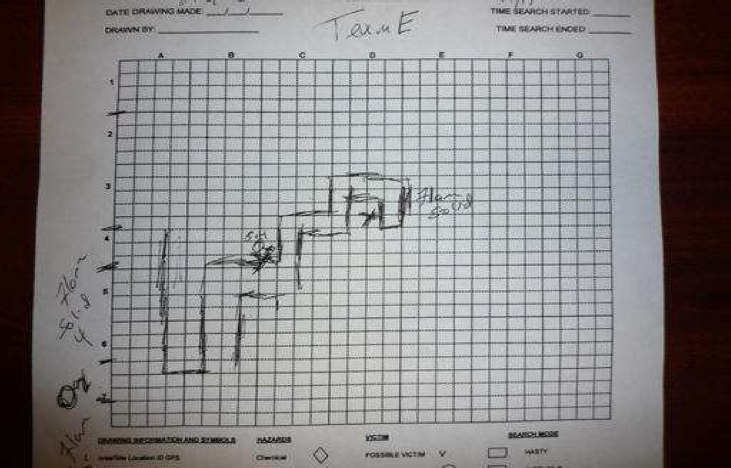
\includegraphics[width=0.65\columnwidth]{figures/map-drawing.jpg}
	}
	\caption{The currently employed workflow requires the \IC\ to draw a two-dimensional map by hand for orientation.}
	\label{fig:workflow:sota}
\end{figure}

\section{Related Work} \label{sec:relatedwork}
\noindent {\bfseries Emergency management.} Much of the visualization-oriented work that is published in the general field of emergency management is concerned with evacuation planning well before any rescue operation has to be performed. Notable work was performed by Reddy \etal, which enables analyzing possible bottlenecks of escape routes~\cite{EuroVA12:13-17:2012}. While algorithms from these areas could be utilized to our benefit, they usually assume perfect walking conditions and a constant structural layout of the building. Ribarsky \etal\ presented a system organizing first responders in intact structures~\cite{Ribarsky:2010}. Kim \etal\ developed a system enhancing the situational awareness of responders using a mobile visual analytics tool~\cite{Kim:2008}. Another related area is the research on visual analysis-supported ensemble steering. While these techniques use ensembles and the visualization to reduce the impact of uncertainty in the input parameters, our system helps the operator to find the best trade-off between the various runs. Ribi\v{c}i\'c \etal\ investigated steering ensembles of flooding simulations using visual analysis~\cite{6280550}. They showed that visual analysis is a valid and useful method for experts to interpret this kind of data. Their idea of generating different measures about a particular flooding inspired our approach to do computation of path ensembles. 

Many existing planning systems deployed nowadays in USAR scenarios are based on 2D representations~\cite{kleiner_et_al_ssrr09,KohlbrecherMeyerStrykKlingaufFlexibleSlamSystem2011,Pellenz2009SMU}. Given the 2D map of the environment, one common approach to path planning is to plan the shortest trajectory and to follow this trajectory stepwise. In harsh environments, however, not the shortest but the safest path can be desirable. Wirth~\etal\ introduced an exploration strategy and path planner that utilizes occupancy grid maps when planning to several targets at the same time~\cite{Wirth2007ETA1}. Consequently, the method selects the safest alternative consisting of target location and path to reach the target. Preliminary extensions towards exploration in 3D were introduced by Dornhege and Kleiner~\cite{dornhege2011frontier}.

%\noindent\textbf{Visual analytics.} There has been work investigating the sense-making process when using visual analytics tools. Gotz \etal\ investigated how to measure insight provenance, a critical measure to judge the quality of reasoning~\cite{Gotz2009}. Roberts presented a state-of-the-art report on how to apply the visual analytics models and techniques using coordinated and multiple views~\cite{roberts2007multipleviews}. Keim \etal\ provide a good overview about the current developments in the field~\cite{keim2010mastering}.

\noindent {\bfseries Point cloud visualization.} As the real-time availability of high resolution point clouds has increased in recent years, there has been much research on rendering techniques for this kind of data. Basic rendering capabilities are provided by the widely used Point Cloud Library which provides a wide array of functionality~\cite{Rusu11ICRA}. Furthermore, there has been work by Richter \etal\ who used a level-of-detail structure to render massive point clouds at high frame rates~\cite{Richter:2010:ORV:1811158.1811178}. Xu \etal\ showed that non-photorealistic rendering techniques can be applied to point cloud data and the resulting contour lines in their rendering inspired our rendering algorithm~\cite{conf/npar/XuC04}. More recently Pintus \etal\ presented a rendering algorithm that enhances features of unstructured point clouds in real time without preprocessing~\cite{Pintus:2011:RRM:2384495.2384513}.

\section{Decision-Making Theory} \label{sec:theory}
Human decision makers in time-constrained situations such as fire fighting tend to evaluate options serially. They attempt to find one viable plan that should work rather than attempting to generate and compare numerous plans in parallel. This theory has been described by Klein and Calderwood~\cite{KleinCalderwood} as Recognition Primed Decision-making (RPD). Initially, human experts look for similarities to previous situations that bring up goals that were relevant, things that were important to monitor, and actions that were possible to pursue. Then, they go through a process of mental simulation to consider whether the actions would work also for the case at hand. They also assess the ongoing situation, looking for violations and confirmations of expectancies, which may require reframing the situation. Klein and Calderwood suggested also that ``displays and interfaces can be centered on decisions rather than around data flows'', emphasizing that systems can be built to enhance the decision process. 

Similarly, the contextual control model (COCOM) describes how people rely on context when making decisions~\cite{hollnagel2005joint}. This theory recognizes that humans sometimes act with plans of lower quality, relying on the environment to make decisions of next steps opportunistically without having a whole plan to reach the end goal. The quality of their control of the situation can be described as scrambled, opportunistic, tactical, or strategic. The scrambled mode refers to decisions made without any idea of what to do. In the opportunistic mode, people rely on cues in the local context to decide their next action. In tactical mode, they have or get an idea of how to achieve their goal --- a plan. In strategic mode, the plan includes coordination with other simultaneous goals. The goal of our system is to lift the quality of control from being opportunistic (as in the current workflow) to being strategic, thus enabling improved decision-making capabilities.

Turning to the granularity of plans, the Extended Control Model (ECOM)~\cite{hollnagel2005joint} describes plans in terms of a tactical level (setting goals), monitoring (making plans and overseeing plans), regulating (managing local resources), and tracking (performing and adjusting actions). This theory can be used to apprise what kind of planning support a system provides.  Moreover, it has been argued by Lundberg \etal\ that in areas such as emergency response it is important to support resiliency: ``Rather than merely selecting a response from a ready-made table, [the system] must adapt and create a suitable response; either by following ready-made plans for adaptation or by making sense of the situation and create responses during the unfolding event''~\cite{Lundberg2012}. Thus, in addition to supporting specific responses that can be foreseen, the system should also support work outside of specific prepared means.

\section{Incident Commander Workflow} \label{sec:workflow}

\graphicspath{{figures/}}
\begin{figure}
\centering
\def\svgwidth{\columnwidth}
\section{Incident Commander Workflow} \label{sec:workflow}

\graphicspath{{figures/}}
\begin{figure}
\centering
\def\svgwidth{\columnwidth}
\section{Incident Commander Workflow} \label{sec:workflow}

\graphicspath{{figures/}}
\begin{figure}
\centering
\def\svgwidth{\columnwidth}
\input{figures/workflow.pdf_tex}
\caption{A schematic timeline overview of the currently employed workflow and our proposed system, showing all events (red) and actions (blue). Utilizing a parallel scanning (yellow) and thus faster and less dangerous exploration, we decrease the overall time-to-rescue.}
\label{fig:workflow:workflow}
\end{figure}

While there is no definition of a rescue team in an USAR incident, in most protocols, for example FEMA~\cite{fema08} or Emergency Management Australia~\cite{em35}, one \IC\ is responsible for a single building and instructs multiple rescue responders inside this building. We will describe the current workflow of the \IC\ first and then propose a visualization-enhanced workflow supported by our system (see Figure~\ref{fig:workflow:workflow}).

\noindent {\bfseries Current workflow.} After arriving at the disaster scene, the first step for the responders is to explore and secure the area outside the collapsed building. No rescuer is allowed to enter the building before it is secured, which can take up to an hour to finish. Then, based on the gathered information, the \IC\ determines valid entry points into the structure and directs rescuers into the collapsed structure to perform reconnaissance. Using constant radio communication, the rescuer inside the building slowly moves forward and reports his progress to the \IC\ who draws a two dimensional map based on that information, as shown in Figure~\ref{fig:workflow:sota}. The rescuer enters an unknown building with unquantifiable risks, like gas leaks or dormant fires, inside. Not only is the two dimensional drawing of an unstructured three dimensional building insufficient and inaccurate, it also does not provide acceptable spatial awareness. This is clearly an example of opportunistic control, where decisions are made opportunistically based on feedback from the environment. The map is made as the rescuer proceeds, inhibiting higher levels of control in the beginning of the path. Although responders may recognize situations, decisions regarding the path to take are limited to the extent of the current exploration and to their view of the local environment. At least initially, therefore, any RPD is restricted to the local environment. Global planning is limited further by the ability of responders to communicate relevant structural information accurately to the \IC.

\noindent {\bfseries Visualization-enhanced workflow.} The initial steps of arriving and exploring the area outside the collapsed structure are the same as in the currently employed workflow. While the responders secure the building, the most time-consuming of the initial tasks, the unmanned robots can be released into the structure and start recording and measuring the inside of the structure and feeding back the information to the \IC\ (the overlapping box in Figure~\ref{fig:workflow:workflow}). The map data from possibly multiple robots is co-registered and the \IC\ inspects the map and determines viable entry points into the structure. The robots' sensors are able to detect most signs of victims using thermal cameras and heart beat detectors~\cite{6027084, Wu12Eulerian}, but as these measurements are uncertain both false positives and false negatives might arise from the data. The same holds true for hazardous environments like fires, gas leaks, structural unsafe areas, chemical spills, or radiation. All data retrieval and preprocessing can be done in parallel while securing the perimeter, so that all information is available when the insertion begins. Based on suggested or selected POIs, the system computes optimal paths through the dataset which the \IC\ can use to direct the rescuers into the building, this time making informed decision about which ways to take, thus drastically reducing time-to-rescue as the rescuers do not have to explore the building to the same extent, but can proceed directly to the POIs. The proposed system applies RPD to the whole situation, extend the number of available cues, and extend planning from local conditions (tracking and regulating) to higher ECOM levels.

When planning the access paths, a variety of factors must be taken into account. The responder has to maintain a safe distance from hazardous environments, avoid overhanging structures, and the ground must be both stable and level. The uncertainty in the data, the varying requirements, and the required expert knowledge of the \IC\ make it unfeasible to derive an algorithm taking all these variables into account. Furthermore, as these variables are extracted from uncertain data, they are difficult to quantify. The \IC\ has to perform trade-offs to choose between alternatives, for example choosing a longer path, which is faster to traverse than a more dangerous, shorter path. These requirements for expert knowledge and decision making, as well as the uncertainty, make the path selection a perfect example demonstrating how the human in the loop can benefit the decision making.

While the \IC\ is instructing the rescuer to follow one chosen path, the rescuer feeds back new information, for example possible victims or new hazards, that he detects. The \IC\ incorporates this information into the application to update the mapping information and paths in real time. This is of high importance as features might not only have been missed by the robots, but detected features might change during the rescue operation. Fires can start or extinguish, subsequent structural collapses can make areas inaccessible, or debris is removed after the initial reconnaissance making previously inaccessible areas available. Although we are designing a system lifting the decision-making to a strategic control, this bears an opportunistic element of planning in the COCOM-sense. However, the system has to support replanning in a strategic control mode to be able to adapt to changing environments.

\caption{A schematic timeline overview of the currently employed workflow and our proposed system, showing all events (red) and actions (blue). Utilizing a parallel scanning (yellow) and thus faster and less dangerous exploration, we decrease the overall time-to-rescue.}
\label{fig:workflow:workflow}
\end{figure}

While there is no definition of a rescue team in an USAR incident, in most protocols, for example FEMA~\cite{fema08} or Emergency Management Australia~\cite{em35}, one \IC\ is responsible for a single building and instructs multiple rescue responders inside this building. We will describe the current workflow of the \IC\ first and then propose a visualization-enhanced workflow supported by our system (see Figure~\ref{fig:workflow:workflow}).

\noindent {\bfseries Current workflow.} After arriving at the disaster scene, the first step for the responders is to explore and secure the area outside the collapsed building. No rescuer is allowed to enter the building before it is secured, which can take up to an hour to finish. Then, based on the gathered information, the \IC\ determines valid entry points into the structure and directs rescuers into the collapsed structure to perform reconnaissance. Using constant radio communication, the rescuer inside the building slowly moves forward and reports his progress to the \IC\ who draws a two dimensional map based on that information, as shown in Figure~\ref{fig:workflow:sota}. The rescuer enters an unknown building with unquantifiable risks, like gas leaks or dormant fires, inside. Not only is the two dimensional drawing of an unstructured three dimensional building insufficient and inaccurate, it also does not provide acceptable spatial awareness. This is clearly an example of opportunistic control, where decisions are made opportunistically based on feedback from the environment. The map is made as the rescuer proceeds, inhibiting higher levels of control in the beginning of the path. Although responders may recognize situations, decisions regarding the path to take are limited to the extent of the current exploration and to their view of the local environment. At least initially, therefore, any RPD is restricted to the local environment. Global planning is limited further by the ability of responders to communicate relevant structural information accurately to the \IC.

\noindent {\bfseries Visualization-enhanced workflow.} The initial steps of arriving and exploring the area outside the collapsed structure are the same as in the currently employed workflow. While the responders secure the building, the most time-consuming of the initial tasks, the unmanned robots can be released into the structure and start recording and measuring the inside of the structure and feeding back the information to the \IC\ (the overlapping box in Figure~\ref{fig:workflow:workflow}). The map data from possibly multiple robots is co-registered and the \IC\ inspects the map and determines viable entry points into the structure. The robots' sensors are able to detect most signs of victims using thermal cameras and heart beat detectors~\cite{6027084, Wu12Eulerian}, but as these measurements are uncertain both false positives and false negatives might arise from the data. The same holds true for hazardous environments like fires, gas leaks, structural unsafe areas, chemical spills, or radiation. All data retrieval and preprocessing can be done in parallel while securing the perimeter, so that all information is available when the insertion begins. Based on suggested or selected POIs, the system computes optimal paths through the dataset which the \IC\ can use to direct the rescuers into the building, this time making informed decision about which ways to take, thus drastically reducing time-to-rescue as the rescuers do not have to explore the building to the same extent, but can proceed directly to the POIs. The proposed system applies RPD to the whole situation, extend the number of available cues, and extend planning from local conditions (tracking and regulating) to higher ECOM levels.

When planning the access paths, a variety of factors must be taken into account. The responder has to maintain a safe distance from hazardous environments, avoid overhanging structures, and the ground must be both stable and level. The uncertainty in the data, the varying requirements, and the required expert knowledge of the \IC\ make it unfeasible to derive an algorithm taking all these variables into account. Furthermore, as these variables are extracted from uncertain data, they are difficult to quantify. The \IC\ has to perform trade-offs to choose between alternatives, for example choosing a longer path, which is faster to traverse than a more dangerous, shorter path. These requirements for expert knowledge and decision making, as well as the uncertainty, make the path selection a perfect example demonstrating how the human in the loop can benefit the decision making.

While the \IC\ is instructing the rescuer to follow one chosen path, the rescuer feeds back new information, for example possible victims or new hazards, that he detects. The \IC\ incorporates this information into the application to update the mapping information and paths in real time. This is of high importance as features might not only have been missed by the robots, but detected features might change during the rescue operation. Fires can start or extinguish, subsequent structural collapses can make areas inaccessible, or debris is removed after the initial reconnaissance making previously inaccessible areas available. Although we are designing a system lifting the decision-making to a strategic control, this bears an opportunistic element of planning in the COCOM-sense. However, the system has to support replanning in a strategic control mode to be able to adapt to changing environments.

\caption{A schematic timeline overview of the currently employed workflow and our proposed system, showing all events (red) and actions (blue). Utilizing a parallel scanning (yellow) and thus faster and less dangerous exploration, we decrease the overall time-to-rescue.}
\label{fig:workflow:workflow}
\end{figure}

While there is no definition of a rescue team in an USAR incident, in most protocols, for example FEMA~\cite{fema08} or Emergency Management Australia~\cite{em35}, one \IC\ is responsible for a single building and instructs multiple rescue responders inside this building. We will describe the current workflow of the \IC\ first and then propose a visualization-enhanced workflow supported by our system (see Figure~\ref{fig:workflow:workflow}).

\noindent {\bfseries Current workflow.} After arriving at the disaster scene, the first step for the responders is to explore and secure the area outside the collapsed building. No rescuer is allowed to enter the building before it is secured, which can take up to an hour to finish. Then, based on the gathered information, the \IC\ determines valid entry points into the structure and directs rescuers into the collapsed structure to perform reconnaissance. Using constant radio communication, the rescuer inside the building slowly moves forward and reports his progress to the \IC\ who draws a two dimensional map based on that information, as shown in Figure~\ref{fig:workflow:sota}. The rescuer enters an unknown building with unquantifiable risks, like gas leaks or dormant fires, inside. Not only is the two dimensional drawing of an unstructured three dimensional building insufficient and inaccurate, it also does not provide acceptable spatial awareness. This is clearly an example of opportunistic control, where decisions are made opportunistically based on feedback from the environment. The map is made as the rescuer proceeds, inhibiting higher levels of control in the beginning of the path. Although responders may recognize situations, decisions regarding the path to take are limited to the extent of the current exploration and to their view of the local environment. At least initially, therefore, any RPD is restricted to the local environment. Global planning is limited further by the ability of responders to communicate relevant structural information accurately to the \IC.

\noindent {\bfseries Visualization-enhanced workflow.} The initial steps of arriving and exploring the area outside the collapsed structure are the same as in the currently employed workflow. While the responders secure the building, the most time-consuming of the initial tasks, the unmanned robots can be released into the structure and start recording and measuring the inside of the structure and feeding back the information to the \IC\ (the overlapping box in Figure~\ref{fig:workflow:workflow}). The map data from possibly multiple robots is co-registered and the \IC\ inspects the map and determines viable entry points into the structure. The robots' sensors are able to detect most signs of victims using thermal cameras and heart beat detectors~\cite{6027084, Wu12Eulerian}, but as these measurements are uncertain both false positives and false negatives might arise from the data. The same holds true for hazardous environments like fires, gas leaks, structural unsafe areas, chemical spills, or radiation. All data retrieval and preprocessing can be done in parallel while securing the perimeter, so that all information is available when the insertion begins. Based on suggested or selected POIs, the system computes optimal paths through the dataset which the \IC\ can use to direct the rescuers into the building, this time making informed decision about which ways to take, thus drastically reducing time-to-rescue as the rescuers do not have to explore the building to the same extent, but can proceed directly to the POIs. The proposed system applies RPD to the whole situation, extend the number of available cues, and extend planning from local conditions (tracking and regulating) to higher ECOM levels.

When planning the access paths, a variety of factors must be taken into account. The responder has to maintain a safe distance from hazardous environments, avoid overhanging structures, and the ground must be both stable and level. The uncertainty in the data, the varying requirements, and the required expert knowledge of the \IC\ make it unfeasible to derive an algorithm taking all these variables into account. Furthermore, as these variables are extracted from uncertain data, they are difficult to quantify. The \IC\ has to perform trade-offs to choose between alternatives, for example choosing a longer path, which is faster to traverse than a more dangerous, shorter path. These requirements for expert knowledge and decision making, as well as the uncertainty, make the path selection a perfect example demonstrating how the human in the loop can benefit the decision making.

While the \IC\ is instructing the rescuer to follow one chosen path, the rescuer feeds back new information, for example possible victims or new hazards, that he detects. The \IC\ incorporates this information into the application to update the mapping information and paths in real time. This is of high importance as features might not only have been missed by the robots, but detected features might change during the rescue operation. Fires can start or extinguish, subsequent structural collapses can make areas inaccessible, or debris is removed after the initial reconnaissance making previously inaccessible areas available. Although we are designing a system lifting the decision-making to a strategic control, this bears an opportunistic element of planning in the COCOM-sense. However, the system has to support replanning in a strategic control mode to be able to adapt to changing environments.

\section{System Overview} \label{sec:overview}
\begin{figure}
    \centering
    \framebox[\columnwidth][c]{
        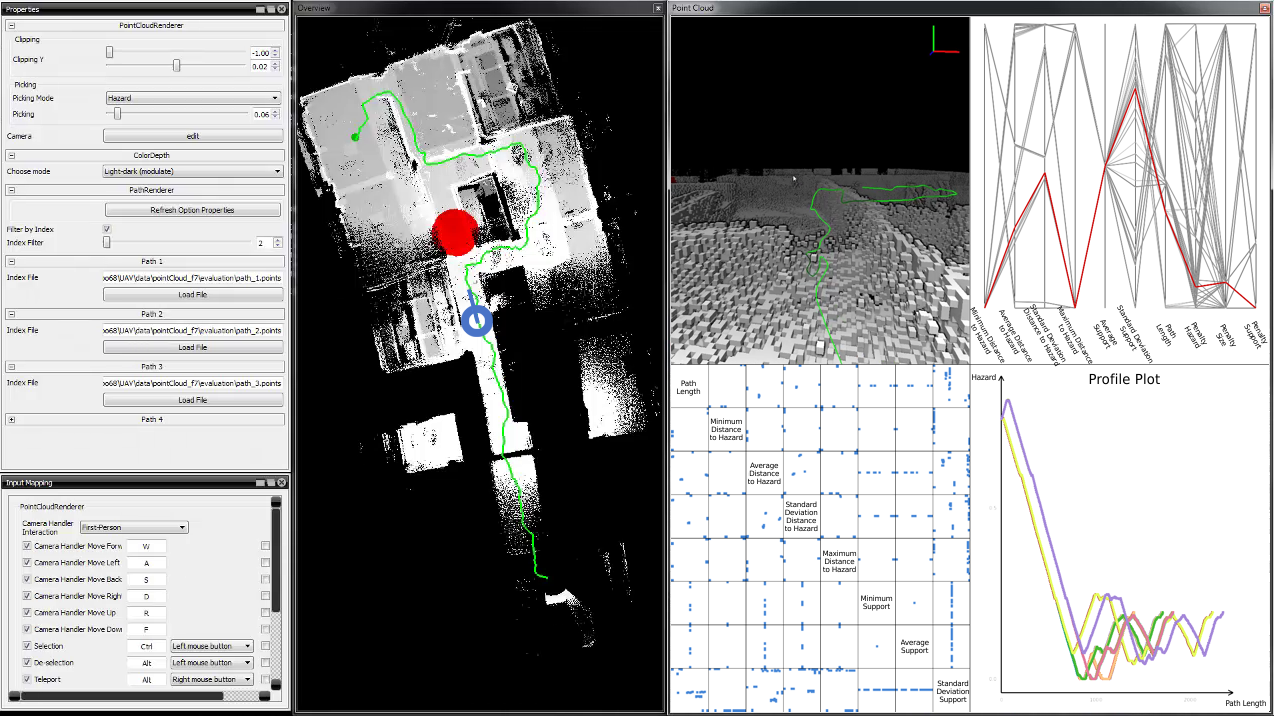
\includegraphics[width=\columnwidth]{figures/fig-overview-system2.png}
    }
    \caption{A screenshot showing our system using usage. The overview map is shown in the middle with the current camera position marked. The right view allows or detailed inspection and navigation. Each subview can be maximized.}
    \label{sec:overview:system}
\end{figure}

In order to fulfil requirement {\bfseries R1}, our system presents the acquired point cloud as an interactive 3D rendering, which preserves occlusion and allows the \IC\ to form a mental model of the structure. In this rendering environment, the \IC\ can seamlessly annotate newly discovered entrances, hazards, and POIs, thus fulfilling requirement {\bfseries R2}. To address requirements {\bfseries R3} and {\bfseries R4}, we provide renderings of the different paths integrated into the 3D rendering as well as separate, in-depth analysis tools.

The following subsections explain the individual parts of the proposed system. The data preprocessing that extracts derived data from the point cloud is described in Section~\ref{sec:overview:precomputation}. The data annotation is illustrated in Section~\ref{sec:overview:classification}. The computation of the ensemble of paths, and the metric used, is described in Section~\ref{sec:overview:path} while Section~\ref{sec:overview:analysis} deals with the support of the analysis of these paths. Section~\ref{sec:overview:rendering} explains the considerations that went into the rendering.

\subsection{Data Preprocessing} \label{sec:overview:precomputation}
\begin{figure*}
    \newlength{\mysize}
    \setlength{\mysize}{0.35\columnwidth}
    \centering
	\subfigure[Hazard field]{
	    \framebox[\mysize][c]{
	        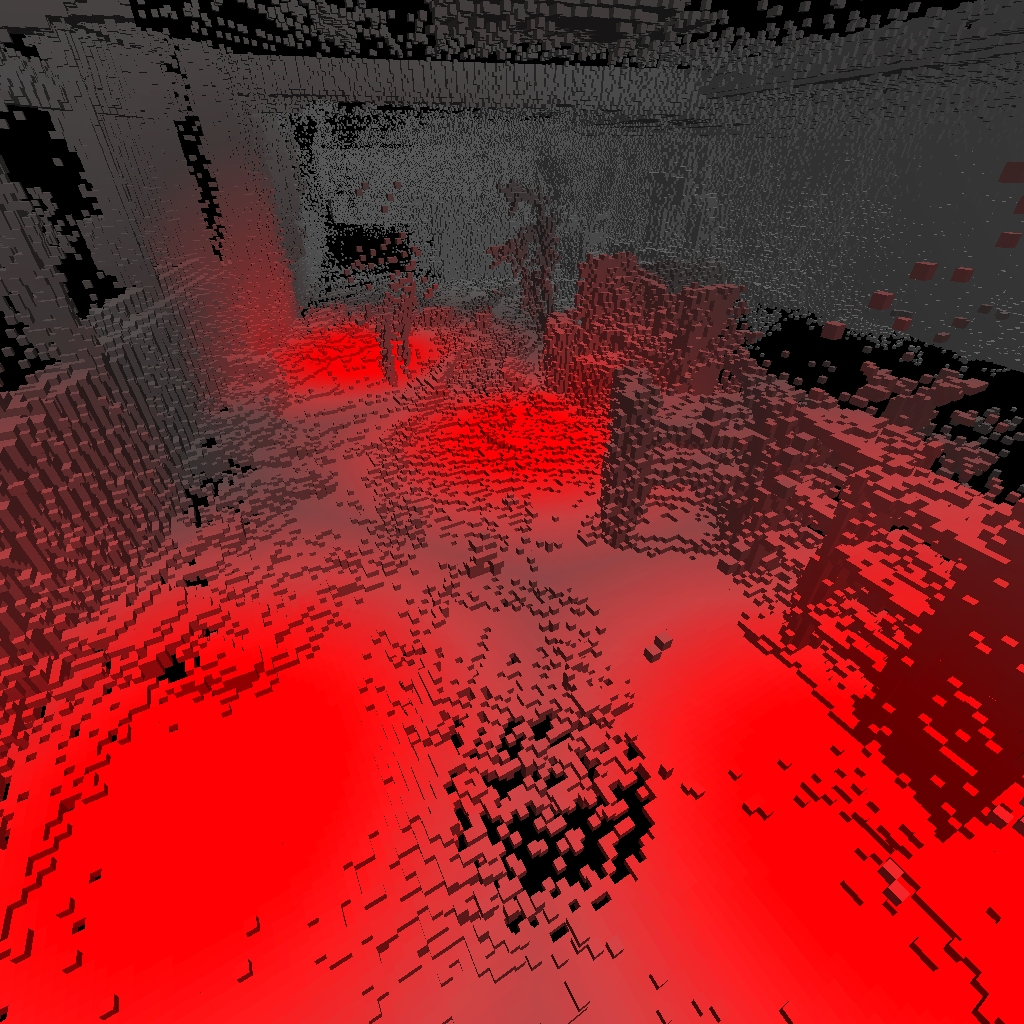
\includegraphics[width=\mysize]{figures/fig-overview-hazardfield.jpg}
	    }
	    \label{fig:overview:precomputation:hazardfield}
	}
	\subfigure[Support field]{
	    \framebox[\mysize][c]{
	        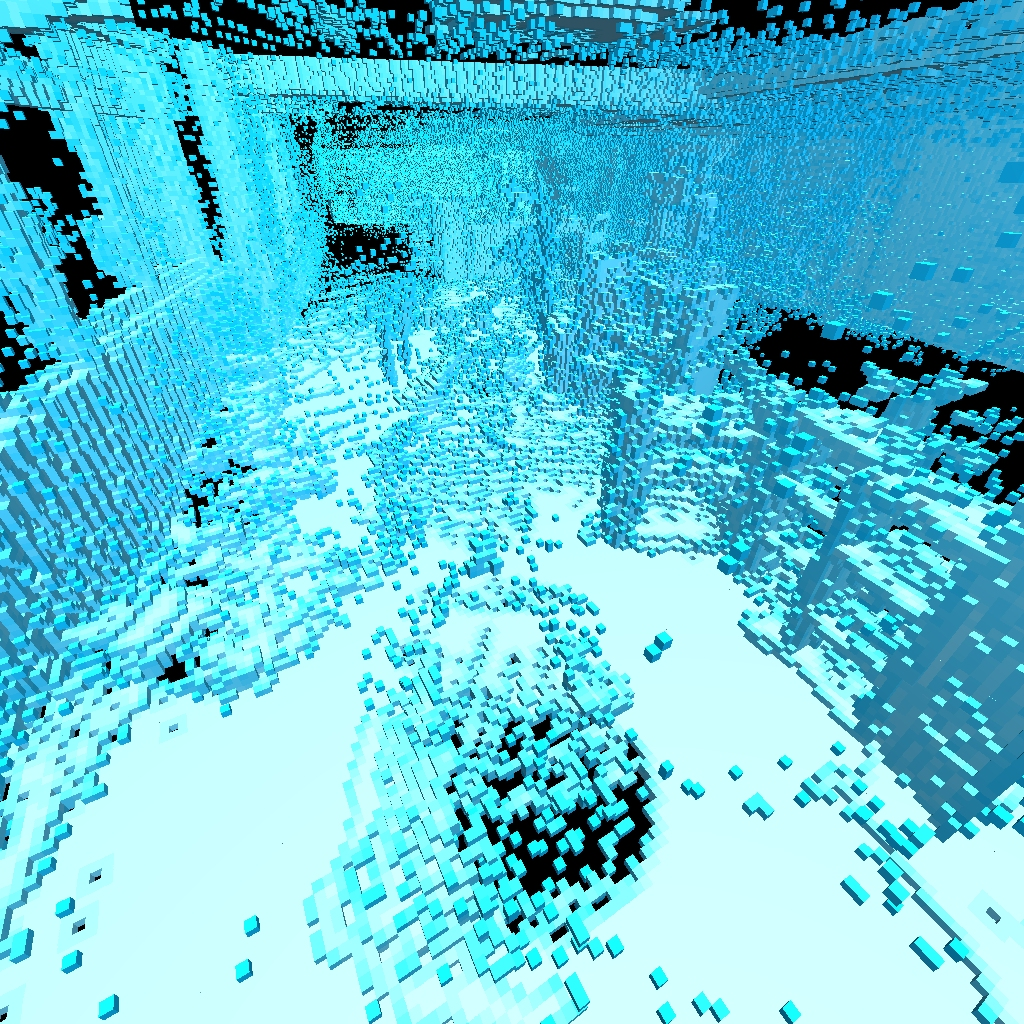
\includegraphics[width=\mysize]{figures/fig-overview-supportfield.jpg}
	    }
	    \label{fig:overview:precomputation:supportfield}
	}
	\subfigure[Occupancy field]{
	    \framebox[\mysize][c]{
	        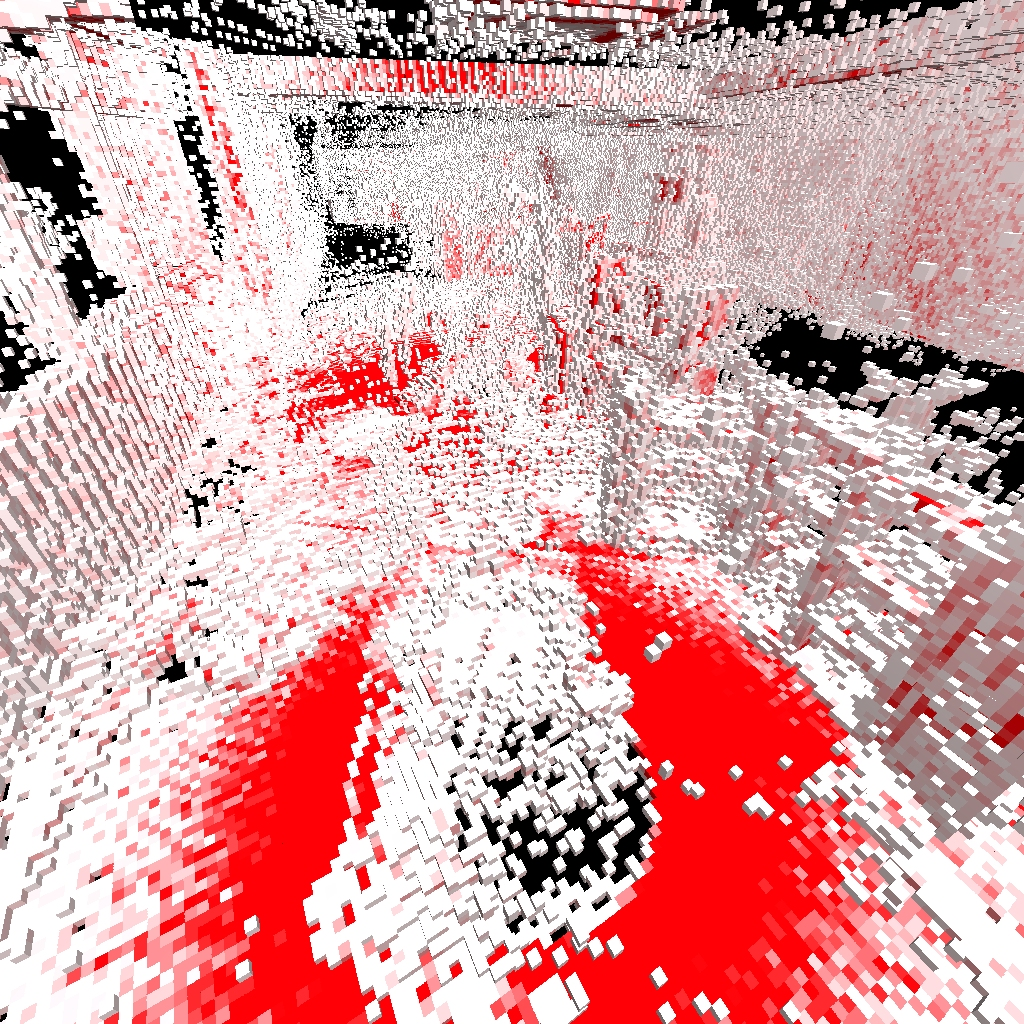
\includegraphics[width=\mysize]{figures/fig-overview-occupancyfield.jpg}
	    }
	    \label{fig:overview:precomputation:occupancyfield}
	}
	\subfigure[Size field]{
	    \framebox[\mysize][c]{
	        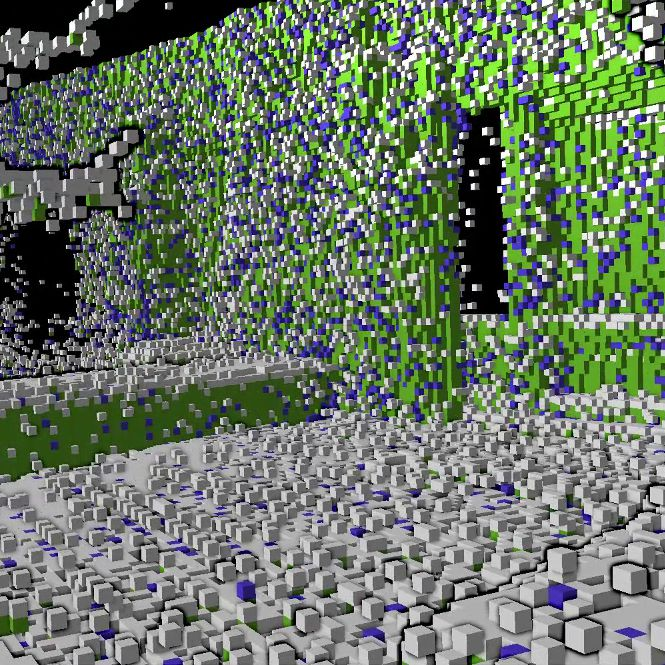
\includegraphics[width=\mysize]{figures/fig-overview-sizefield.jpg}
	    }
	    \label{fig:overview:precomputation:sizefield}
	}
	\caption{Three of the derived attributes are mapped to the individual voxels and are shown: (a) closest distance to hazard, (b) level of support, (c) occupancy, or data density, and (d) the availability of space above each voxel.}
    \label{fig:overview:precomputation}
\end{figure*}

\noindent {\bfseries Scan conversion.} The data retrieved from the unmanned robots is an unstructured 3D point cloud of the interior of the collapsed building. The resolution of the scan is highly dependent on the allotted scanning time as well as the employed scanner. One issue with point rendering is missing occlusion information. To avoid this problem, we perform a binning of the point cloud to obtain an axis-aligned voxel data structure. The necessary voxel size is highly dependent on the scan resolution of the robot, as it is a trade-off between resolving smaller details versus increasingly noisy data. In our test case, voxel sizes of $5$cm were sufficient with regard to this trade-off. The resulting grid-based data structure contains one voxel for all bins with the occupancy exceeding a certain threshold. In our approach, we discard every voxel that only depends on a single measurement point, since this is likely due to measurement noise. From this point on we refer to a \emph{point} in the original point cloud and to a \emph{voxel} in the binned point cloud.

\noindent {\bfseries Parameter derivation.} Derived attributes are computed for the voxel data, which are subsequently used to determine a set of viable rescue paths and to support filtering of these paths. We compute a \emph{distance field} (Figure~\ref{fig:overview:precomputation:hazardfield}) that denotes the distance to the closest hazard points, weighted by severity, for each voxel. Let $\mathbf{i}$ be the current voxel, $H$ the set of hazard points, and $H^{\mathbf{i}}_s$ the normalized severity for $\mathbf{i}$, then the hazard field is given by: $h(\mathbf{i}) = \min_\mathbf{j}(\mathrm{L}_2(\mathbf{i}, H^\mathbf{j}) \cdot H^\mathbf{j}_s)$. The \emph{support field} (Figure~\ref{fig:overview:precomputation:supportfield}) shows the available supporting area for each voxel. This value determines if there is enough floor available for a responder to walk unhindered. The voxel neighborhood in the plane perpendicular to the gravity axis is considered as that plane coincides with horizontal surfaces. The \emph{occupancy field} (Figure~\ref{fig:overview:precomputation:occupancyfield}) denotes the number of  points each voxel is based on. A higher occupancy means that the voxel contains more points in the original point cloud data and thus provides a higher certainty. The occupancy can be increased by longer scan rates and better scanning technology. The \emph{size field} (Figure~\ref{fig:overview:precomputation:sizefield}) shows for each voxel if a rescuer can fit into the space above without squeezing. We calculate two size values, one with the rescuer standing up and a second while crouching.

To compute viable paths, we need orientation information to be able to exclude paths that would be to steep for a rescuer. We utilize data normals in order to indicate the orientation of structures of interest. We investigated two sensible measures for determining the normal direction at each voxel. In the first method we compute the least-squares fitted plane based on all the points that a voxel covers. The normal of the resulting plane is used as the normal for the voxel. The second method performs a least-squares fit of the neighborhood of the voxel to determine the principal direction of the plane. In our tests we found that the first method results in greater stability provided higher occupancy.

\subsection{Data Annotation} \label{sec:overview:classification}
With respect to requirement {\bfseries R2} it is essential for the \IC\ to be able to classify and annotate the data. Each voxel can belong to one of five classes. \emph{Unclassified} is the default type for all voxels. \emph{Start} voxels are entry points, which the \IC\ has declared as accessible. This means that each path can start from any of these set of points. \emph{POI} voxels are denoted, either by the robots or by the \IC, to be destination points for a path. \emph{Hazard} voxels have been declared as dangerous due to, for example, an ongoing fire or gas leak. Each hazard area has a severity that denotes how important it is to avoid it. \emph{Forbidden} voxels can only be declared by the user and are areas completely out of reach for traversal. These points are used when, for example, a corridor collapses and is not accessible anymore.

The \IC\ can modify the classification for each voxel by interacting with the rendering of the point cloud. He can either modify a single point or perform a radius-based selection of all nearby points close to the selection. 

\subsection{Path Computation} \label{sec:overview:path}
For the path computations we make use of the widely used A* algorithm~\cite{4082128}. It is a best-first search algorithm that uses the L$_2$ distance as a heuristic to estimate the distance to the target. The algorithm works as follows. For the current point $x$ all unvisited neighboring points $y_i$ have the estimated remaining distance calculated. This value is the sum of the cost to reach $x$, the cost to move from $x$ to $y_i$, and the estimated cost to reach the target. These points are inserted into an open list and the point with the lowest cost is chosen as the next valid point; the current point is then removed from the open list and marked as visited. For a comprehensive description of the algorithm we refer the reader to~\cite{AStar}.

The metric determines the cost of moving from one point to its neighbor. Thus, it is possible to compute several optimal paths by changing the metric that is used for the A* algorithm. While it is possible to change the metric during the computation, we did not include this into our system as the resulting complexity in interaction would be prohibitive for the \IC. The metric that is used in our system is composed of several, weighted submetrics that are summed up to yield the metric $m$

\begin{eqnarray*}
m & = & \textrm{distance}(\mathbf{p},\mathbf{q}) + w_h \cdot \textrm{hazard}(\mathbf{q}) + w_s \cdot \textrm{size}(\mathbf{q}) + \\
  & & w_n \cdot \textrm{normal}(\mathbf{q},\varphi) + w_{sup} \cdot \textrm{support}(\mathbf{q},n)
%m = & w_d \cdot distance(p,q) + w_h \cdot hazard(p,q) + \\
%  & w_n \cdot normal(p,q,angle) + w_s \cdot size(p,q,type) + \\
%  & w_o \cdot overhang(p,q) + w_{sup} \cdot support(p,q,area,n)
\end{eqnarray*}

\noindent where $w_{h,n,s,sup}$ are the weights that are varied between different runs, of the path computation. $\mathbf{p}$ is the current point, and $\mathbf{q}$ is the point under consideration.

The function $\textrm{distance}(\mathbf{p},\mathbf{q})$ calculates the L$_2$ distance between points $\mathbf{p}$ and $\mathbf{q}$ with the result in standard units. $\textrm{hazard}(\mathbf{q})$ returns the hazard severity. $\textrm{size}(\mathbf{q})$ is a binary function that determines if there is enough space above the voxel $\mathbf{q}$. The $\textrm{normal}(\mathbf{q},\varphi)$ function computes the surface normal for $\mathbf{q}$ and returns a normalized, linear response between the maximum allowed deviation $\varphi$ and the gravity vector. The $\mathrm{support}(\mathbf{q},n)$ value is dependent on the amount of supporting voxels in the area around the point $\mathbf{q}$. This area depends on the voxel size and should cover an area of about 50cm. The $n$ parameter is a threshold determining how many voxels are needed to consider $\mathbf{q}$ supported.

For different parameter combinations the optimal path from the entry points to the POIs is computed. While many of those paths will take different ways through the point cloud, some might not arrive at the POI and are discarded. For example if $w_h$ is set to infinity and the only possible path passes through a hazard field there exists no valid path. If there are multiple POIs the \IC\ can choose to compute paths that visit each of the POIs in turn. The resulting travelling-salesman problem can be solved heuristically~\cite{4569756}.

Global information is calculated for each path; for instance, each path segment provides information about the distance to the closest hazard, while the path stores the minimum, maximum, and average distance together with the standard deviation to allow for in-depth analysis by the \IC. Furthermore, the total length of the path is calculated. 

\subsection{Visual Path Analysis} \label{sec:overview:analysis}
\begin{figure*}
    \newlength{\mysize}
    \setlength{\mysize}{0.32\textwidth}
    \centering
	\subfigure[Parallel Coordinates Plot]{
	    \framebox[\mysize][c]{
	        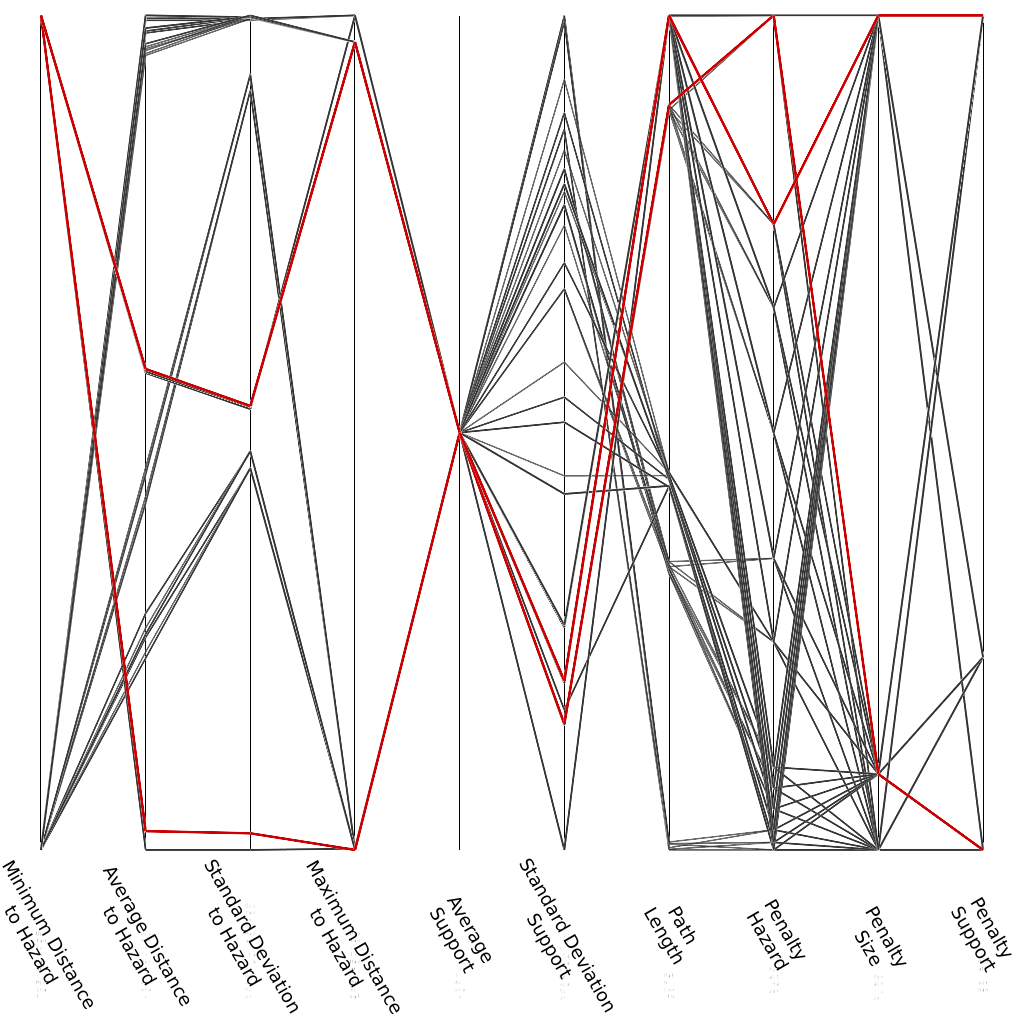
\includegraphics[width=\mysize]{figures/fig-analysis-pcp.png}
	    }
	    \label{fig:overview:analysis:pcp}
	}
	\subfigure[Scatter Plot Matrix]{
	    \framebox[\mysize][c]{
	        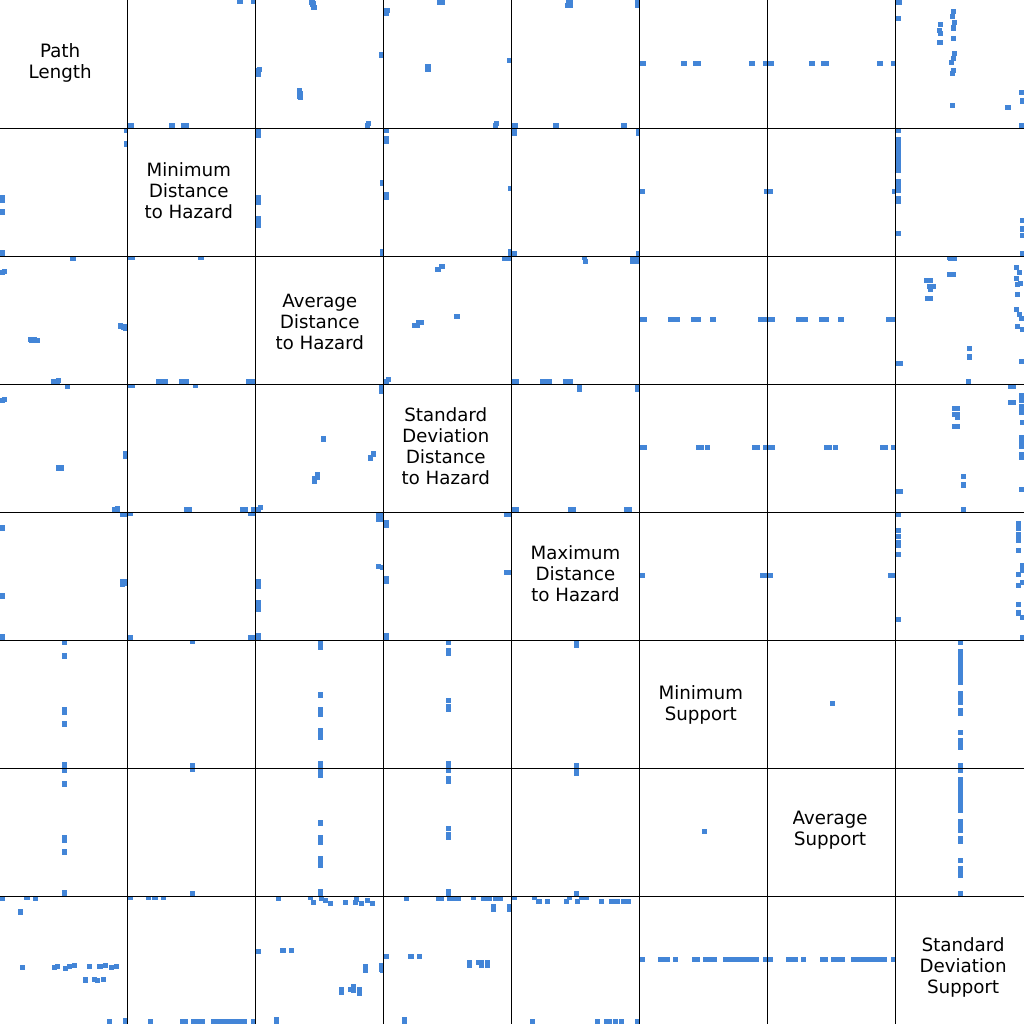
\includegraphics[width=\mysize]{figures/fig-analysis-scatter.png}
	    }
	    \label{fig:overview:analysis:scatter}
	}
	\subfigure[Profile Plot]{
	    \framebox[\mysize][c]{
	        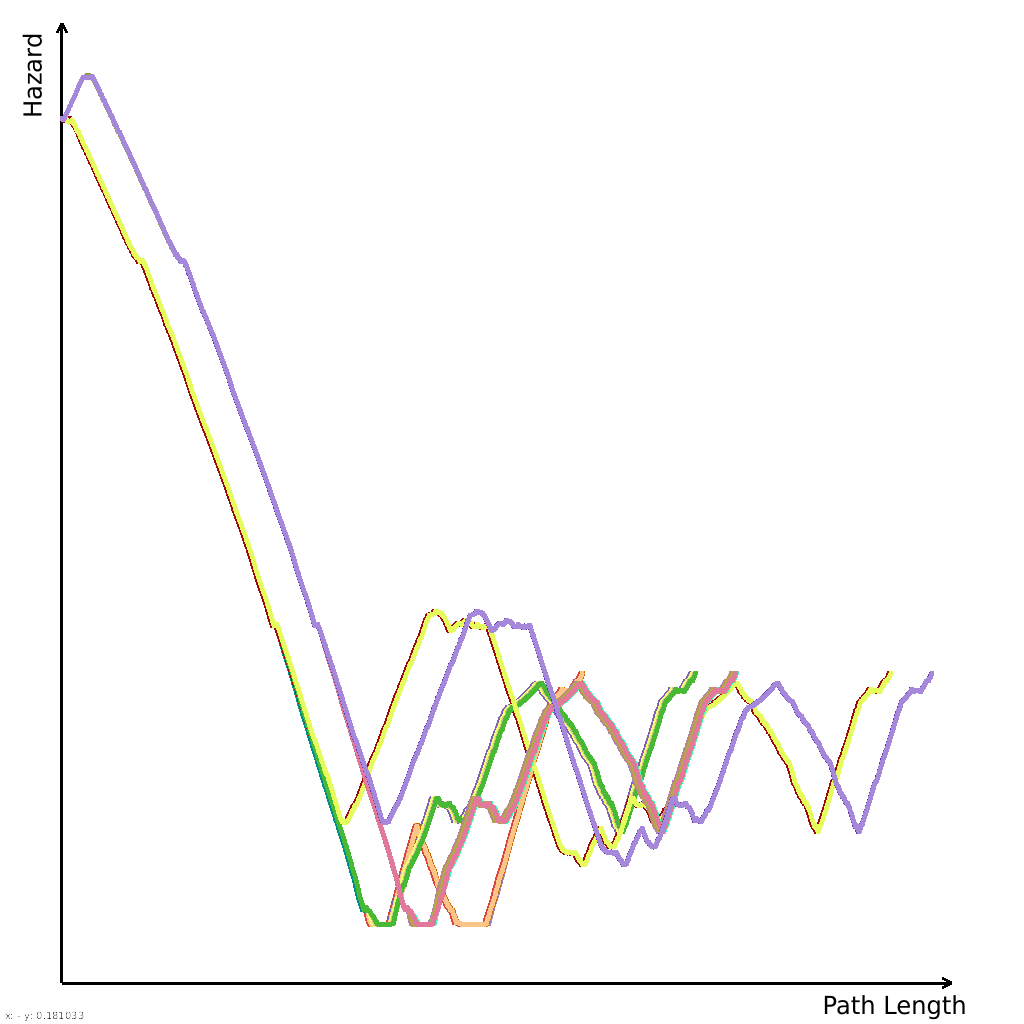
\includegraphics[width=\mysize]{figures/fig-analysis-profile.png}
	    }
	    \label{fig:overview:analysis:profile}
	}
    \caption{Screenshots of the analysis views in our system. (a) parallel coordinates plot with one of the paths selected. (b) scatter plot matrix depicting the correlations of all attributes. (c) distance to the closest hazard over path length.}
\end{figure*}

In order to enable informed trade-offs between all computed paths and selecting one suitable path, it is essential to provide detailed information about the various paths in a way that is easy to interpret. In this section we will explain the different views accessible by the \IC\ to gain a deeper understanding of the data. All views utilize the same brushing and linking features.

The \IC\ can use these methods to filter the large number of computed paths so that he can make an informed decision about an optimal trade-off. These trade-offs depend on the specific situation and experience of the \IC\ but include travel distance versus proximity to hazards or inclination of the walking surface versus available support among others. Because the exact details of the trade-offs depend on the \IC, we provide adaptive tools to filter and analyze the data according to information the \IC\ requests. This allows him to make full use of his knowledge in a strategic decision making scenario.

\subsubsection{Parallel Coordinates Plot} \label{sec:overview:analysis:pcp}
Parallel Coordinates Plots (PCP)~\cite{146402} are a visualization technique to inspect multidimensional data. It is very well suited to detect regularities and patterns in the data and deviations from these patterns and also enhances interactive exploration of data sources~\cite{Tory05aparallel}.

Figure~\ref{fig:overview:analysis:pcp} shows the PCP in our system with each computed path represented by one line. The axes are grouped into \emph{derived attributes}, like path length, minimal distance to hazard, average distance to hazard, or standard deviation of support, and \emph{path parameters} that were used to compute the path in question. While the first group is used to perform the necessary trade-off between paths, the second group is primarily used to filter the data. The \IC\ can select which attributes and parameters are visible in the PCP.  Through exploration of parameters, the \IC\ can move from mental simulation of alternatives, to simulation supported by the decision support system, thus amplifying RPD. The ability to explore trade-offs between alternative paths should facilitate a strategic COCOM decision mode, for the targeting ECOM level. In addition to filtering of paths, which is replicated in all other views, the \IC\ can select a path in this view and the selection is also linked in the system. Detecting previously unknown correlations and the ability to filter large parts of the data quickly helps to fulfil requirements {\bfseries R3} and {\bfseries R4}.

\subsubsection{Scatter Plot Matrix} \label{sec:overview:analysis:scatter}
The PCP is primarily used for those aspects that we foresee that the \IC\ wants to compare frequently. However, in line with the literature on resilience engineering~\cite{Lundberg2012} we also provide comparisons that cannot be foreseen in advance. Therefore we present attributes in a Scatter Plot Matrix (SPLOM), where each variable is given a row of scatter plots that show relations to all other variables. It allows the \IC\ to make comparisons opportunistically, zooming in on the required comparisons if needed. Each individual scatter plot shows the correlation between two attributes and can be used by the \IC\ to verify known relationships or discover new interactions~\cite{Li2008}. In addition, paths selected in this view are linked to the other views providing a consistent representation of the available paths. Figure~\ref{fig:overview:analysis:scatter} shows the SPLOM during usage.

\subsubsection{Profile Plot} \label{sec:overview:analysis:profile}
PCP and SPLOM are useful to inspect attributes that are valid for the path as a whole. In order to enable detailed analyses of values that change along the path, we include a profile plot. This is a variation of a line plot with different attributes over the path length enabling the \IC\ to spot outliers among the paths. This view makes it easy to compare the paths with regard to the chosen variable, as minima and maxima over all paths are easy to detect. Furthermore, it allows the \IC\ to spot irregularities along the path due to measurement errors, which would present themselves as single spikes. Having the possibility to detect these spikes, it is possible to fix the measurement errors and come to a more accurate path description. In Figure~\ref{fig:overview:analysis:profile} hazard distance profiles for a set of already filtered paths are shown. 

\subsection{Rendering} \label{sec:overview:rendering}
\noindent {\bfseries Point Cloud Rendering.} Rendering the unfiltered point cloud proved to be insufficient in early tests as missing depth cues and surface occlusion inhibited the necessary immersion. A voxelized representation is beneficial, as rendering each voxel using axis-aligned boxes solves the occlusion problem immediately (Figure~\ref{fig:teaser:1}). Holes appear in the rendering only in cases with very sparse data. To increase the spatial awareness, we apply an illumination technique to the rendering, where the lighting is based on the face normal of the voxel, rather than the normal of the voxel as computed in Section~\ref{sec:overview:precomputation}. We use the face normal as it is completely stable and constant for a given surface, thus making surfaces easier to detect. The \IC\ can add clip planes, for example to remove ceilings, to deal with unwanted occlusion in the scene.

\noindent {\bfseries Path Rendering.} In order for the user to understand the spatial relationship of the paths, it is useful and necessary to show the paths embedded in the rendering. Since the paths are computed based on the center points of the voxels, it is necessary to increase the $y$ value of each control point by at least half the voxel size in $y$ direction. In our experiments, we found that increasing it by about 2--3 times the voxel size produces a good visual result without looking too detached.

The \IC\ can select different coloring to inspect the stored information about the paths. Since the rendering view can become very cluttered, it is possible for the user to select a path in the rendering, which highlights that path in all other linked views and desaturates all other paths. Thus, it is possible to inspect the exact behavior of a few paths without distraction and also allows the user to reduce the number of considered paths very quickly.

Rather than relying on a mental simulation of the situation, the \IC\ can use a virtual walkthrough to inspect whether a plan will actually work. This walkthrough can either be interactively steered by the \IC\ or the camera can follow a chosen path automatically. Through looking at the information, the \IC\ can use his own experience to judge whether a path is likely to be passable.
\section{Implementation} \label{sec:implementation}

In this section, we will describe the details necessary to reproduce this work. We used the OpenMP framework~\cite{660313} for most of the preprocessing and path computation and achieved a speedup that is very close to linear.

\noindent {\bfseries Data Preprocessing.} The input data for this step is the acquired and co-registered point cloud from the autonomous robots. Each point in the point cloud stores its position in a global coordinate system as well as additional information, for example a color value or results from other scanners. Based on this data the voxel binning and filtering is performed. A user-defined voxel size in standard units is prescribed and the points of the point cloud are assigned to their closest voxel center. The number of points per voxel is the occupancy, as in Section~\ref{sec:overview:precomputation}. The filtering step removes all voxels with an occupancy below a defined threshold; in our case $1$. This generates a second point cloud containing only the valid voxel centers. In a following step all necessary fields are computed for the voxel point cloud, like normals, size restrictions or support. These operations are done in parallel for each voxel and do not require any intercommunication, thus making the parallelization near-optimal. For the Fukushima dataset with 35 million points, the full precomputation takes between one and two minutes on a four core machine.

\noindent {\bfseries Rendering.} The 3D rendering is performed on the preprocessed point cloud using OpenGL 4. The positions of the occupied voxel centers are stored in a vertex buffer object and rendered with a single \texttt{glDrawArrays} command. The different fields~(Figure~\ref{fig:overview:precomputation}) are stored in VBOs and attached as vertex attributes. The vertex shader performs packing of these values to increase the performance when the vertices are pushed through the pipeline. Although this operation reduces the dynamic range for the fields to 8 bits, the visual difference is minimal. As the size of the binning is known, a geometry shader constructs the vertices for an axis-aligned bounding box around each center, thus rendering the front faces of the boxes without the need for additional storage on the GPU. With all optimizations we achieve frame rates of at least $20$fps for our datasets.

\noindent {\bfseries Path Computation.} As described in Section~\ref{sec:overview:path} we use the A* algorithm with our composite metric $m$ to generate an ensemble of paths. The four weights $w_{h,n,s,sup}$ and two values $angle$ and $n$ in the metric span a six-dimensional parameter space. We sample this space on a regular grid and compute a path for each parameter configuration. High parallelism is possible as all paths are computed independently of one another. For each path the fields are calculated and stored alongside an ordered list of voxels that path passes through. For each voxel, the submetric decision criteria are stored as well. In our experiments we sampled the parameter space at $\approx 10^5$ positions and the computations required about a minute on a four core machine with $3$GHz. With respect to the parallelism an increase in cores will lead to a linear decrease in computation time. 
\section{Application Case---Fukushima Daiichi Reactor} \label{sec:cases}
\begin{figure}
    \centering
    \framebox[0.4\columnwidth][c]{
        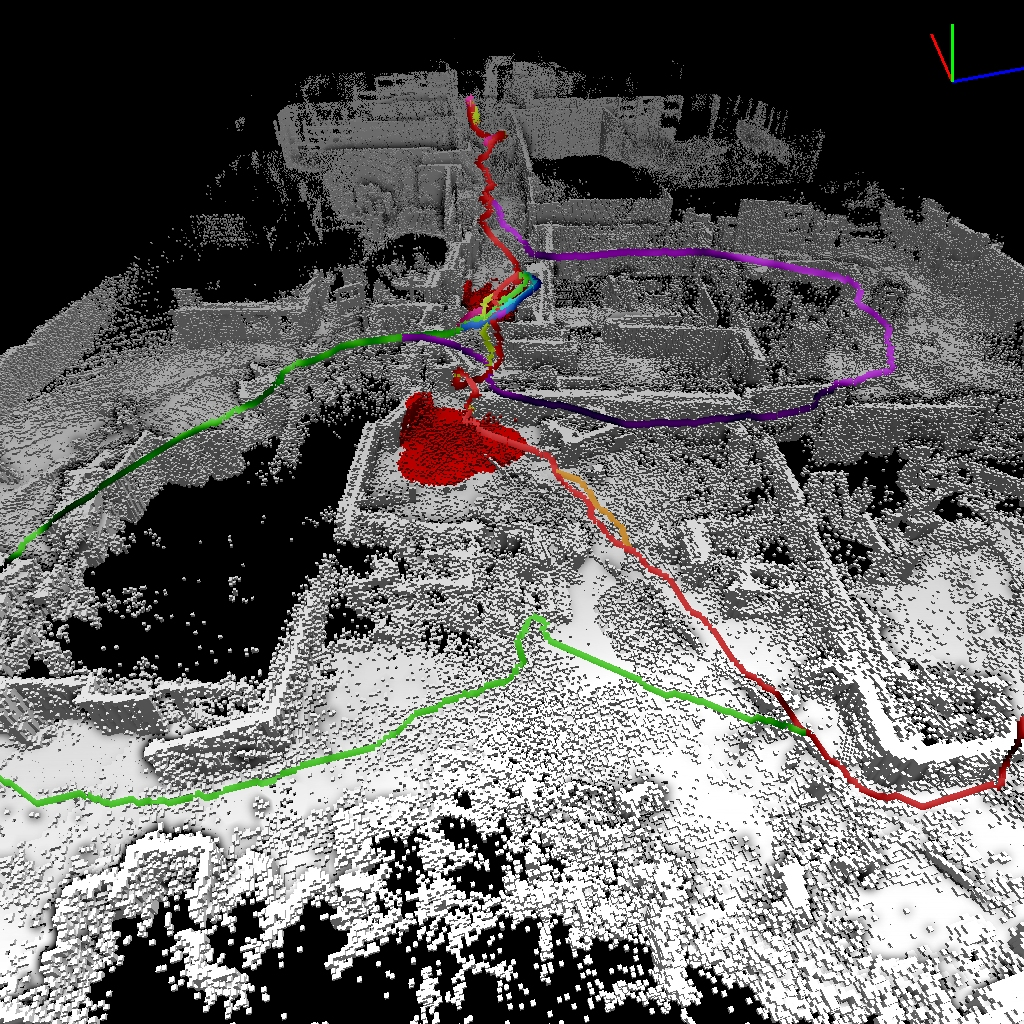
\includegraphics[width=0.4\columnwidth]{figures/fig-analysis-rendering.jpg}
    }
    \caption{The different paths are shown integrated into the rendering to provide a better awareness of the alternatives.}
    \label{fig:overview:analysis:paths}
\end{figure}
As autonomous robots are not yet used in emergency situations, it was not possible to obtain a dataset from a real-world disaster area. Hence we like to thank the IRIDeS, the CREATE, and the IRS institutes for their cooperation in retrieving three scans from the Fukushima Daiichi nuclear reactor in the aftermath of the 2011 meltdown. The equipment that was used to produce the scans are described in~\cite{journals/jfr/NagataniKOOYTNYKFK13}. As there had been hydrogen explosions and collapses in the building, it proved to be a valid and useful simulated real-world application case to test our proposed system.

Figure~\ref{fig:teaser:3} shows an overview of the scanned area with the selected entry area on the top in cyan, and the POI in green, on the bottom. No hazards were detected by the robots during the acquisition. The task was as follows: the \IC\ needs to find the shortest path between the entry and the POI. While traversing along the path, an imaginary rescuer would detect two hazard clouds (visible in red in Figure~\ref{fig:teaser:3}) and the system has to be able to react to this changing information as by requirement {\bfseries R2}.

Figure~\ref{fig:overview:analysis:paths} shows the rendering with all computed paths after the second hazard has been discovered. There is one class of paths (shown in purple) that evades the first hazard and another class (shown in green) that evades the second hazard. The parallel coordinates plot (Figure~\ref{fig:overview:analysis:pcp} makes it possible to detect a path that belongs to both classes as it has a maximum in the minimal distance to the hazard, while having a long path length (the selected path). In this snapshot of the SPLOM, Figure~\ref{fig:overview:analysis:scatter} shows the relationship between path length and the standard deviation of the support area and shows that the shorter the paths tend to pass through more unstable areas. The profile plot in Figure~\ref{fig:overview:analysis:profile} shows the prominence of the purple path as well.

\section{Evaluation} \label{sec:evaluation}
We performed a qualitative evaluation of our system with three experts. One of the experts is a field leading researcher in emergency informatics, the two others are full-time employees at the Federal Agency for Technical Relief (THW) in Germany, one of them being a station officer. As the overall number of experts in the field is not high enough to perform thorough quantitative user studies, we decided to perform a quantitative, informal study. We prepared an expressive video showing the functionalities of the system navigating the preprocessed point cloud and annotating a start point and a POI. Then, an optimal path was computed between these points, which had to be modified as hazardous environments became known. The test scenario is based on the application case presented in Section~\ref{sec:cases}. Figures~\ref{fig:teaser:2}, ~\ref{fig:teaser:3}, and~\ref{fig:teaser:4} show still shots from this video. Afterwards, we asked the experts three open questions with the request to answer as elaborate as possible. The questions and their answers were:

\noindent \textbf{"Is it helpful to display the paths and does this representation provide additional information?"} One of the experts was very convinced about the usefulness of the system and suggested many other application areas close to his daily work, which would benefit from our system, such as a fire brigade trying to extinguish a fire in a building. The limited visibility in such an environment would benefit greatly from the system according to the expert. The other two experts were positive, but not as enthusiastic.

\noindent \textbf{"Would you like to use this system in addition, or as a replacement, to your current tools?"} Two of the respondents would like to use the system in their workflow and were very positive about it. One of them could not see it as an addition, as they do not currently use any computer system in their work. This expert further noted that it would be important to know how long it would take to generate these representations to perform a cost/benefit analysis. The third expert would like to try out the system in a controlled test environment before making any predictions.

\noindent \textbf{"Is it easier to analyze the scene using our rendering method [as compared to a point-based rendering]?"} Although the replies from all respondents were positive, each suggested a useful improvement to the system. One expert thought it would be useful for 2D navigation and thought that a color picture of the building would have helped. The second expert would have liked to see a multi-story building in the video to be able to detect rubble and damaged ceilings to assess the usefulness towards detecting this kind of dangerous situations. The last respondent thought it was easier to analyze the data, but wished for a higher resolution of the voxelized point cloud data (see Figure~\ref{fig:teaser:1} for a dataset with the same voxel size).

From the answers received we can draw the conclusion that all of the experts liked the system, but wanted to test it in a real-world application case to see how well it performs. This is in line with our future plans of performing a thorough scenario-based evaluation to receive more feedback to improve the system.
\section{Conclusions and Future Work} \label{sec:conclusion}
In this paper, we presented a comprehensive system that optimizes the workflow of an incident commander when dealing with urban search \& rescue missions in cases where the initial reconnaissance of a collapsed structure is performed using unmanned robots. We analyzed the workflow from a visualization perspective and designed a linked multiple-view system that allows the \IC\ to effectively annotate a three-dimensional rendering of a filtered point cloud. Based on this enriched data, our system computes and analyzes a large number of paths. The resulting information is visualized for the \IC , who can then select a path that is optimal according to his experience and knowledge. To investigate the effectivity of the proposed system we have conducted a study with expert users. The resulting positive feedback makes us confident that the proposed system has the potential to improve future search \& rescue planning missions.

For future work we like to perform a thorough in-use evaluation workshop with domain experts using a real-world scenario. This will provide us with valuable direct feedback to improve the usability of the system. Furthermore, we will investigate the applicability of adaptive or stochastic sampling methods, like Monte-Carlo methods, on the high-dimensional parameter space for path computation.

%\section*{Acknowledgements}
%This work was partly supported by grants from the Excellence Center at Link\"oping and Lund in Information Technology (ELLIIT) and the Swedish e-Science Research Centre (SeRC), as well as VR grant 2011-4113. We would like to thank the anonymous reviewers for their valuable feedback and the experts for taking their time to take part in the evaluation. The presented concepts have been realized using the Voreen framework (www.voreen.org).

%% if specified like this the section will be ommitted in review mode

\newpage
\bibliographystyle{eg-alpha-doi}
%%use following if all content of bibtex file should be shown
%\nocite{*}
\bibliography{bibliography}
\end{document}
